\chapter{Experiments}
\label{chap:experiments}

This chapter presents the experimental results for the studied algorithm settings. 
We begin by examining how the lower-bound fitness can be estimated from the input instances. 
Next, we analyze the elitist genetic algorithm. In particular, we compare evolutionary ordering of boxes with an ordering based on box volume, 
and we study the effect of letting the algorithm select a placement heuristic for each box instead of using a single fixed heuristic. 
After that, we investigate how mutation and memetic hill-climbing influence the performance of the algorithm. 
Finally, we evaluate the baseline hill-climbing approach and test whether introducing probabilistic acceptance improves its results.

\section{Fitness Lower Bound}

To better interpret the quality of obtained solutions, we introduce a lower bound estimate of the fitness function defined in Section~\ref{sec:fitness-function}. 
The fitness function consists of two parts: the first is the number of opened containers, and the second measures how well the least filled container is utilized. 

Firstly, we consider the lower bound induced by the volume constraint. 
Dividing the total volume of all boxes by the volume of a single container gives the minimum amount of container space that must be used. 
The integer part of this ratio corresponds to fully utilized containers, while the fractional part describes how much of the last container is occupied. 
Since the fitness function consists of the number of opened containers and a penalty based on the occupancy of the least filled container, 
one additional container must be accounted for in the volume-based bound. Therefore, the volume-based lower bound of the fitness value is given by:

\[
L_{\mathrm{volume}} = \frac{\sum_{i=1}^{N} \mathrm{V}(s_i)}{\mathrm{V}(S)} + 1.
\]

Similarly, we can introduce a lower bound induced by the weight constraint. We divide the total weight of all boxes by the maximum allowed container weight:

\[
L_{\mathrm{weight}} = \frac{\sum_{i=1}^{N} w_i}{W_{\max}} + 1.
\]


The final lower bound is obtained as the maximum of the volume-based and weight-based bounds:
\[
L = \max \left(L_{\mathrm{volume}}, L_{\mathrm{weight}}\right).
\]

Although this bound does not capture geometric packing constraints, it provides a consistent theoretical reference based solely on resource feasibility.

The average lower bound fitness values for the original, medium, and heavy datasets, 
across all classes and numbers of boxes, are presented in Table~\ref{tab:lower-bound}.
The lower bound increases for the medium dataset and even further for the heavy dataset, 
which clearly demonstrates that the solutions become increasingly constrained not only by volume, 
but also by weight.

\begin{table}[htbp]
\centering
\caption{Comparison of lower bound fitness across datasets (average values)}
\label{tab:lower-bound}
\begin{tabular}{|c|c|c|c|c|}
\hline
Class & $N$ & Original & Medium & Heavy \\ \hline
class 1 & 100 & 10.53 & 12.42 & 15.28 \\ \hline
class 1 & 150 & 15.99 & 19.06 & 23.57 \\ \hline
class 1 & 50  & 6.31  & 7.34  & 8.93  \\ \hline
class 2 & 100 & 7.14  & 8.36  & 10.20 \\ \hline
class 2 & 150 & 10.16 & 12.00 & 14.75 \\ \hline
class 2 & 50  & 4.23  & 4.86  & 5.82  \\ \hline
class 3 & 100 & 5.76  & 6.71  & 8.14  \\ \hline
class 3 & 150 & 8.43  & 9.93  & 12.16 \\ \hline
class 3 & 50  & 3.57  & 4.04  & 4.81  \\ \hline
class 4 & 100 & 13.78 & 16.46 & 20.14 \\ \hline
class 4 & 150 & 21.22 & 25.23 & 31.07 \\ \hline
class 4 & 50  & 7.32  & 8.47  & 10.31 \\ \hline
\end{tabular}
\end{table}

\section{Elitist Genetic Algorithm Experiments}

For the elitist algorithm, we primarily adopt the parameter settings proposed by Gonçalves and Resende \cite{goncalves2013}, 
as shown in Table~\ref{tab:ega-set-hyperparameters}, while the remaining parameters are currently set to zero.

\begin{table}[htbp]
\centering
\caption{Elitist Genetic Algorithm Hyperparameters Setting}
\label{tab:ega-set-hyperparameters}
\begin{tabular}{|l|l|}
\hline
$M$ & $30 \times N$ \\ \hline
$G$ & 300 \\ \hline
$p_E$ & 0.1 \\ \hline
$p_R$ & 0.15 \\ \hline
$p_C$ & 0.70 \\ \hline
\end{tabular}
\end{table}

\subsection{Influence of Placement Heuristics and Box Ordering}

This section examines the combined influence of placement heuristics 
and box ordering on the performance of the algorithm. 
In this set of experiments, we consider only datasets without weights.

We compare two approaches to selecting placement heuristics: 
using a single default heuristic (Max Distance), as in the original work by Gonçalves and Resende \cite{goncalves2013}, 
and allowing the evolutionary algorithm to choose a heuristic for each box from the set defined in 
Section~\ref{sec:placement-heuristics}. 
At the same time, we consider two ordering strategies: 
an ordering determined by the evolutionary algorithm, also inspired by the original work of Gonçalves and Resende \cite{goncalves2013}, 
and a predefined ordering based on descending box volume.

The results are summarized in Table~\ref{tab:combined-results}. 
Each row represents the average fitness of the best solution found for a given dataset type and number of boxes, 
while the evolutionary progress for all four settings, together with the lower bound and the hill-climbing baseline, is illustrated in Figure~\ref{fig:final-original}.
Overall, allowing the evolutionary algorithm to select placement heuristics significantly improves performance across all settings. 
The influence of box ordering is more nuanced. 
For the structured datasets (classes 1--3) in the \emph{All Heuristics} setting, the evolutionary ordering performs slightly better for the smaller instances with 50 boxes, 
while the volume-based ordering becomes slightly better for the larger instances with 150 boxes, 
since it reduces the search space when the instance size grows. 
For the medium-sized instances with 100 boxes, the two strategies are comparable. 
For the random dataset (class 4), evolutionary ordering consistently yields the best results. 
In the \emph{Max Distance} setting, where the placement heuristic is fixed, the results for datasets 1--3 are 
generally similar for evolutionary and volume-based ordering, since the search space is already restricted by the single heuristic. 
Even in this setting, however, evolutionary ordering remains better for class 4 in all instance sizes.

Based on these observations, all subsequent experiments use the setting 
with evolutionary selection of placement heuristics, unless stated otherwise.

\begin{table}[htbp]
\centering
\caption{Comparison of placement heuristics and box ordering for the elitist algorithm on the dataset without weights}
\label{tab:combined-results}
\begin{tabular}{|c|c|c|c|c|c|}
\hline 
Class & $N$ 
& \shortstack{All \\ Evol.} 
& \shortstack{All \\ Volume} 
& \shortstack{Max Dist. \\ Evol.} 
& \shortstack{Max Dist. \\ Volume} \\ \hline
class 1 & 100 & \textbf{11.92} & 11.93 & 12.30 & 12.33 \\ \hline
class 1 & 150 & 18.74 & \textbf{18.71} & 19.28 & 19.20 \\ \hline
class 1 & 50  & \textbf{7.29}  & 7.31  & 7.37  & 7.41  \\ \hline
class 2 & 100 & 7.88  & \textbf{7.88}  & 8.10  & 8.09  \\ \hline
class 2 & 150 & 11.70 & \textbf{11.65} & 11.93 & 11.97 \\ \hline
class 2 & 50  & \textbf{4.61}  & 4.65  & 4.69  & 4.65  \\ \hline
class 3 & 100 & \textbf{6.17}  & \textbf{6.17}  & 6.32  & 6.32  \\ \hline
class 3 & 150 & 9.50  & \textbf{9.48}  & 9.76  & 9.75  \\ \hline
class 3 & 50  & \textbf{3.84}  & 3.86  & 3.88  & 3.88  \\ \hline
class 4 & 100 & \textbf{16.10} & 16.21 & 16.19 & 16.26 \\ \hline
class 4 & 150 & \textbf{24.49} & 24.52 & 24.91 & 25.04 \\ \hline
class 4 & 50  & \textbf{8.57}  & \textbf{8.57}  & 8.69  & 8.75 \\ \hline
\end{tabular}
\end{table}


\subsection{Impact of Mutation and Memetic Search}
This section evaluates the effect of incorporating mutation operators and hill-climbing memetic 
search into the algorithm. To identify suitable parameter settings, we performed a grid search over 
the memetic and mutation parameters listed in Table~\ref{tab:mutation-memetic-parameters}. 

The results show that hill-climbing memetic search does not improve the solution quality in practice. 
In most cases, the results are identical to those obtained without memetic enhancement, 
while the runtime increases due to the additional evaluation of individuals. 
For this reason, the hill-climbing component is not recommended and is kept disabled in the remaining experiments.

We also tested memetic search only on elite individuals, instead of applying it to offspring. 
In this setting, the results were even worse, since non-elite individuals had fewer opportunities 
to surpass the elites, which were further improved by memetic search.

Regarding mutation, the setting $p_M = 0.01$ slightly improves the results for the smallest instances with 50 boxes. 
However, for larger instances, mutation consistently degrades performance. 
This is expected, since the same mutation probability affects a larger number of genes as the instance size increases, making higher mutation rates overly disruptive in larger problems. 
Nevertheless, even for lower values $p_M = 0.003$ and $p_M = 0.005$, which should in principle mitigate this effect, degradation of performance is still observed.

The results are summarized in Table~\ref{tab:mutation-results}, which reports only the small instances with 50 boxes.

\begin{table}[htbp]
\centering
\caption{Grid search over mutation and memetic hyperparameters}
\label{tab:mutation-memetic-parameters}
\begin{tabular}{|c|c|}
\hline
Parameter & Tested values \\ \hline
$I_{HC}$ & 1, 2, 5 \\ \hline
$p_{HC}$ & 0.003, 0.005, 0.01 \\ \hline
$p_M$ & 0.003, 0.005, 0.01 \\ \hline
\end{tabular}
\end{table}

\begin{table}[htbp]
\centering
\caption{Effect of mutation ($p_M = 0.01$) on small instances (50 boxes)}
\label{tab:mutation-results}
\begin{tabular}{|c|c|c|c|}
\hline
Class & No Mutation & Mutation ($p_M = 0.01$) \\ \hline
class 1 & 7.29 & 7.26 \\ \hline
class 2 & 4.61 & 4.59 \\ \hline
class 3 & 3.84 & 3.81 \\ \hline
class 4 & 8.57 & 8.54 \\ \hline
\end{tabular}
\end{table}

\subsection{Influence of Box Weights}

In this section, we investigate how assigning weights to boxes affects the results. 
We again compare the evolutionary ordering of boxes with the volume-based ordering, as in the unweighted dataset. 
In addition, we introduce a heuristic that orders boxes according to their weight.
The experiments are conducted separately on the medium and heavy datasets. 
As in the previous experiments, we use evolutionary selection of placement heuristics, since it performed best on the unweighted dataset.

The convergence curves for the medium dataset, together with the lower bound and the hill-climbing baseline, are shown in Figure~\ref{fig:final-medium}. 
The corresponding results for the heavy dataset are shown in Figure~\ref{fig:final-heavy}. 

Increasing the importance of box weight acts as a strong additional constraint on the packing process. 
As a result, the differences between the three ordering strategies become very small, and the convergence behaviour of the evolutionary ordering, volume-based ordering, and weight-based ordering is nearly identical. 
This is consistent with the fact that box weights were generated from the box volumes, so both heuristics capture largely the same underlying structure of the instances. 
 
Overall, the solutions converge very quickly. 
For the smallest instances with 50 boxes, convergence often occurs within the first 100 generations. 
For the larger instances with 100 and 150 boxes, convergence is typically reached by generation 300, and in many cases the solutions even match the lower bound. 
This effect is especially visible for classes 2 and 3, while class 4, which is unstructured, converges more slowly. 

To compare the overall evolutionary progress across the original, medium, and heavy datasets, Figure~\ref{fig:elitist-weight-comparison} shows the corresponding convergence curves. 
For the comparison of these three strategies, the evolutionary ordering is used as the reference ordering in the corresponding plots. 
An interesting pattern emerges at the beginning of the evolution: the original and medium datasets produce very similar fitness values when the solution is still random, which suggests that the dominant constraint is initially the box volume. 
However, as the evolutionary search progresses, the medium dataset converges earlier because the maximum-weight constraint starts to dominate. 
This is in contrast to the heavy dataset, where it is already apparent at the beginning of the search that random solutions perform noticeably worse than on the original and medium datasets, indicating that the weight constraint is the primary limitation from the very start. 
The heavy dataset therefore exhibits the strongest feasibility pressure. 

Overall, the results confirm that box weight acts as a strong feasibility constraint, and that the volume-based and weight-based heuristics produce very similar behaviour because of the way the datasets were generated.

\begin{figure}[htbp]
    \centering
    \makebox[\textwidth][c]{%
        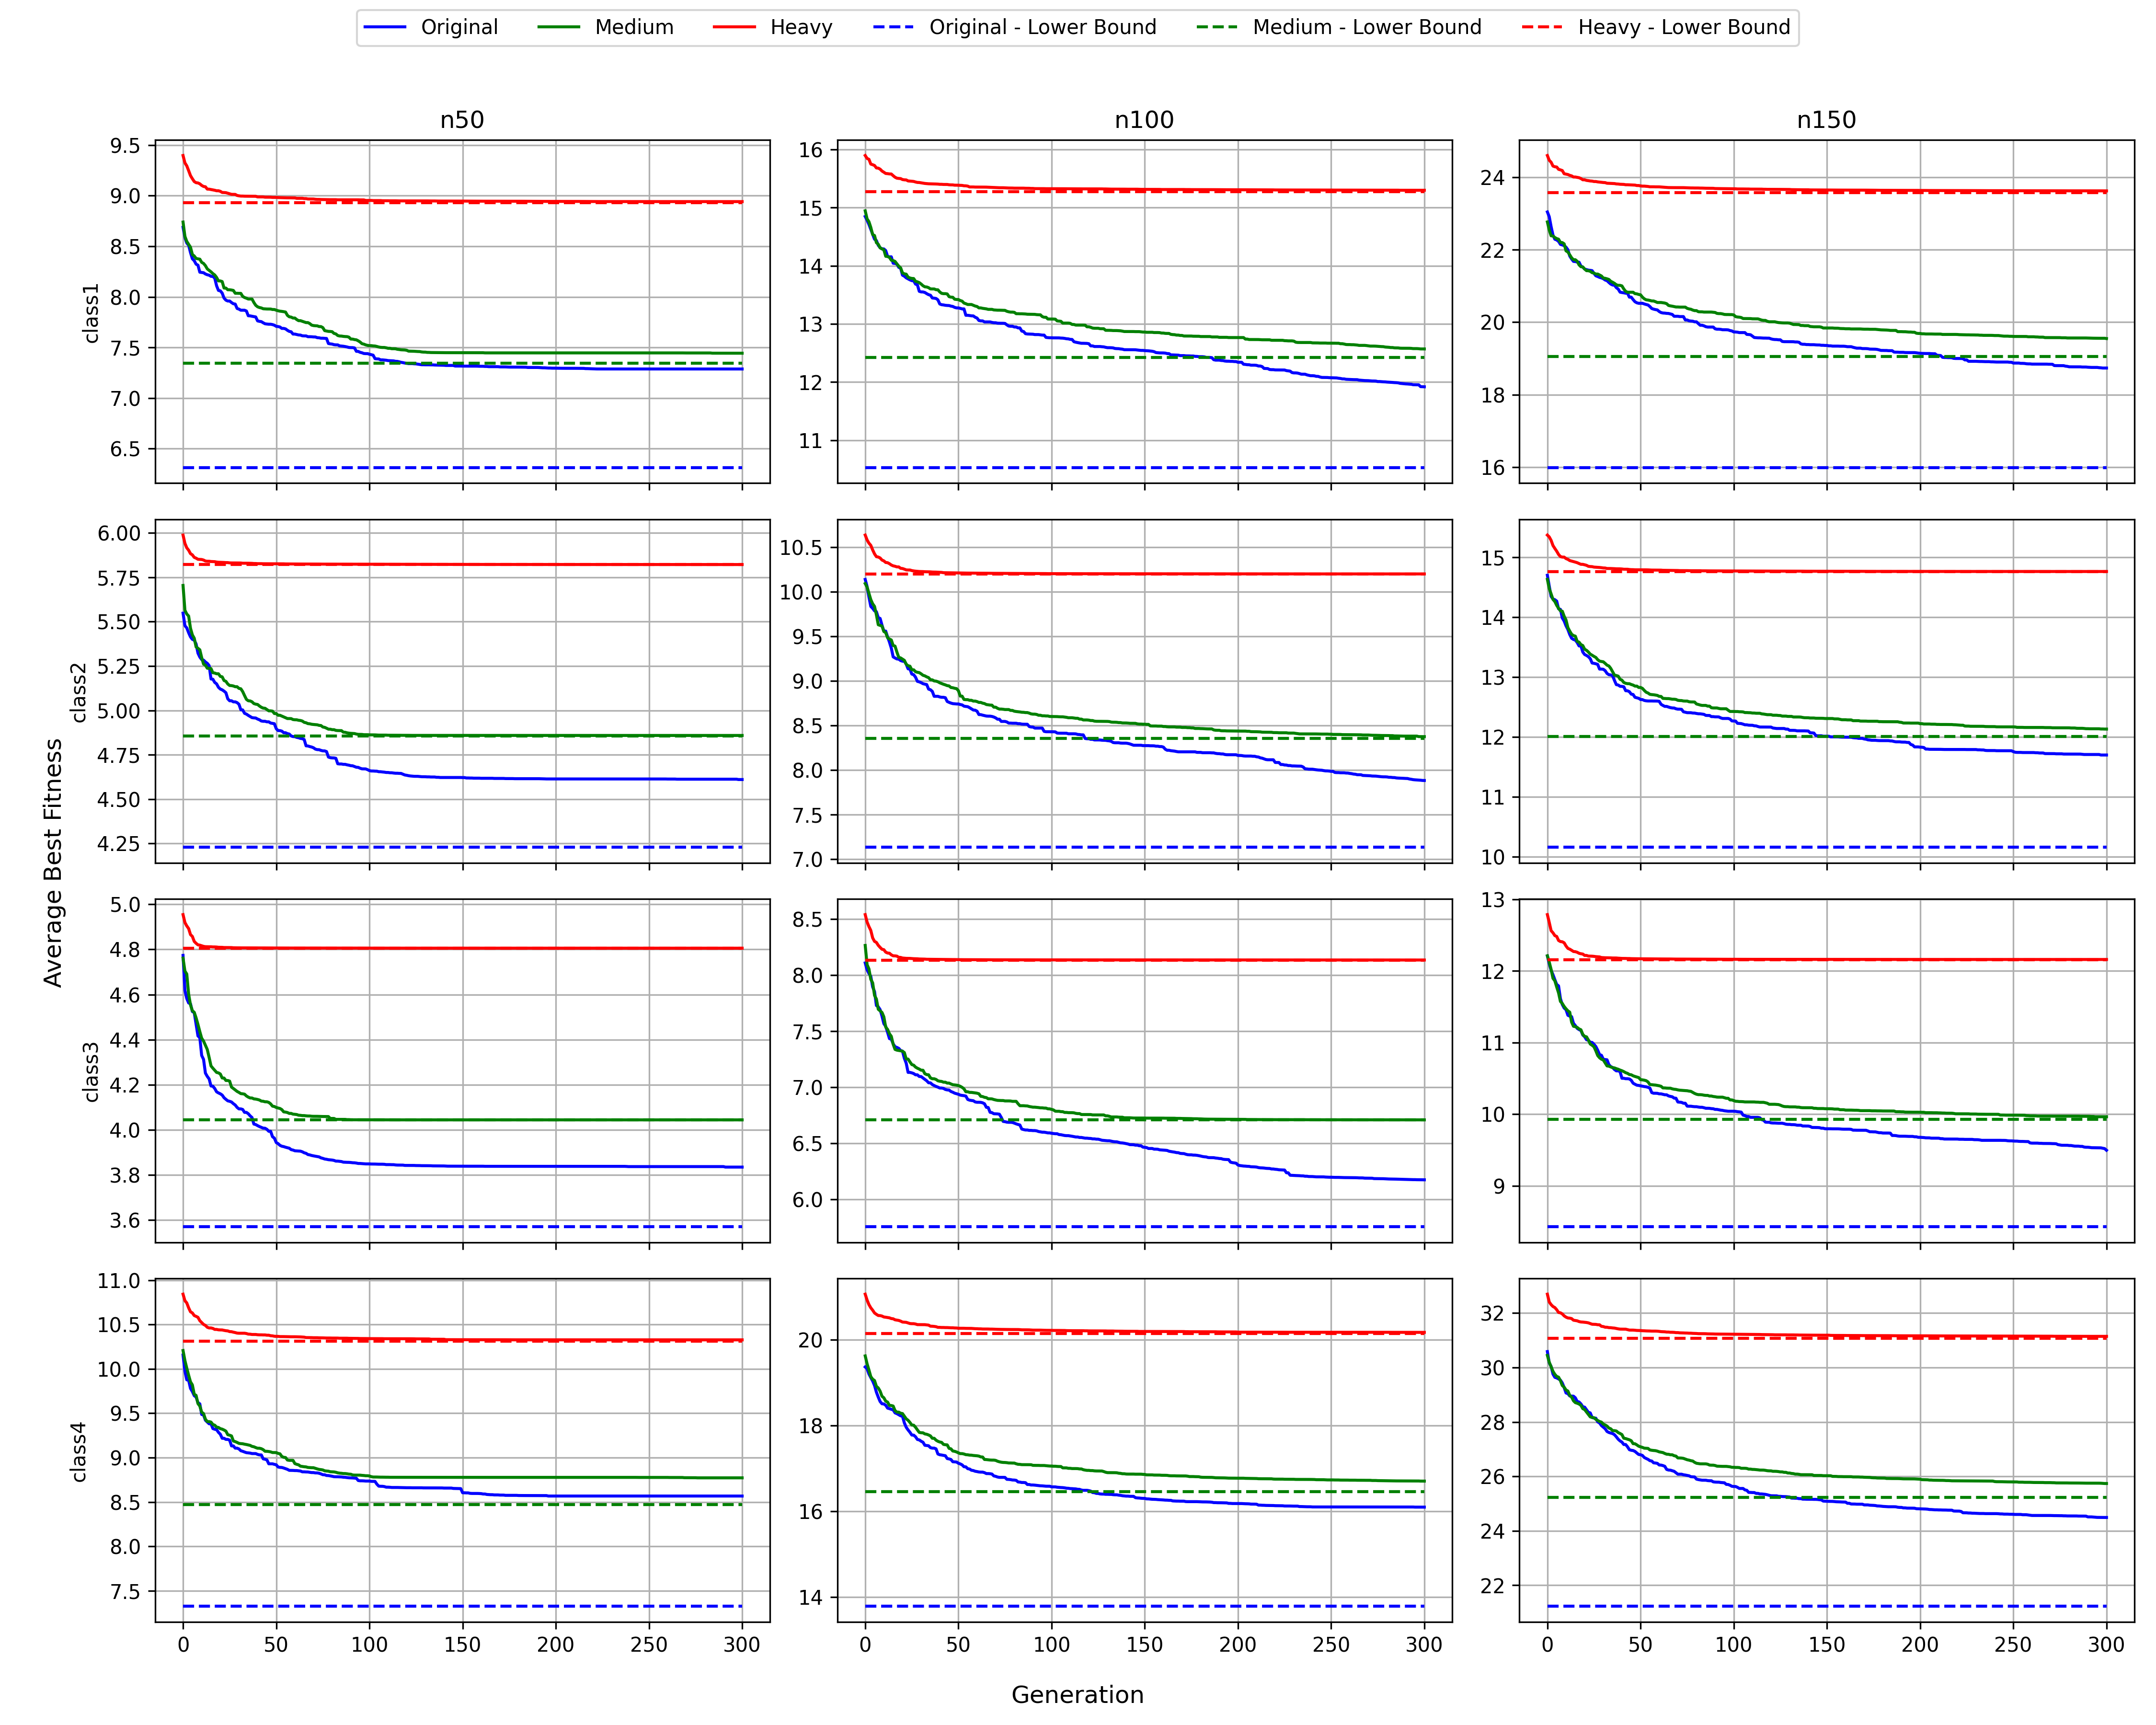
\includegraphics[width=1.2\textwidth]{img/elitist-weights.png}%
    }
    \caption{Comparison of evolutionary progress across the original, medium, and heavy datasets 
    using the elitist algorithm with evolutionary ordering.}
    \label{fig:elitist-weight-comparison}
\end{figure}

\section{Probabilistic Hill Climbing}

This section discusses the results of the hill-climbing baselines used in our experiments. 
We first evaluate simple hill climbing, obtained as the special case of probabilistic hill climbing with $p_A^{(0)} = 0$, and then examine whether allowing a non-zero probability of accepting worse solutions can improve the results.

For both baselines, we performed a grid search over parameter settings chosen so that the pairs $(M,G)$ correspond to approximately the same computational budget: $(30,300)$, $(60,150)$, and $(90,100)$. 
We considered mutation probabilities $p_M \in \{0.005, 0.01\}$. 
For probabilistic hill climbing, we additionally tested initial acceptance probabilities $p_A^{(0)} \in \{0.80, 0.50, 0.20, 0.10\}$ and decay coefficients $\alpha \in \{0.98, 0.985, 0.99\}$. 
The minimum acceptance probability was fixed at $p_{\min}=0$.

The parameter grids for simple hill climbing and probabilistic hill climbing are summarized in Tables~\ref{tab:hc-parameters} and~\ref{tab:phc-parameters}. 
The best configurations for both baselines are summarized in Table~\ref{tab:hc-best-config}.

We use evolutionary selection of placement heuristics throughout this section instead of the Max Distance heuristic, as it performed best in the elitist genetic algorithm experiments.

\begin{table}[htbp]
\centering
\caption{Grid search over hill climbing hyperparameters}
\label{tab:hc-parameters}
\begin{tabular}{|c|c|}
\hline
Parameter & Tested values \\ \hline
$(M,G)$ & $(30 \times N,300)$, $(60 \times N,150)$, $(90 \times N, 100)$ \\ \hline
$p_M$ & 0.005, 0.01 \\ \hline
$p_A^{(0)}$ & 0 \\ \hline
$\alpha$ & 0 \\ \hline
$p_{\min}$ & 0 \\ \hline
\end{tabular}
\end{table}

\begin{table}[htbp]
\centering
\caption{Grid search over probabilistic hill climbing hyperparameters}
\label{tab:phc-parameters}
\begin{tabular}{|c|c|}
\hline
Parameter & Tested values \\ \hline
$(M,G)$ & $(30 \times N, 300)$, $(60 \times N, 150)$, $(90 \times N, 100)$ \\ \hline
$p_M$ & 0.005, 0.01 \\ \hline
$p_A^{(0)}$ & 0.80, 0.50, 0.20, 0.10 \\ \hline
$\alpha$ & 0.98, 0.985, 0.99 \\ \hline
$p_{\min}$ & 0 \\ \hline
\end{tabular}
\end{table}

\begin{table}[htbp]
\centering
\caption{Best hyperparameter configurations for hill climbing baselines}
\label{tab:hc-best-config}
\begin{tabular}{|l|c|c|}
\hline
Parameter & Hill Climbing & Probabilistic Hill Climbing \\ \hline
$(M,G)$ & $(30 \times N, 300)$ & $(30 \times N, 300)$ \\ \hline
$p_M$ & 0.01 & 0.01 \\ \hline
$p_A^{(0)}$ & 0 & 0.10 \\ \hline
$\alpha$ & 0 & 0.98 \\ \hline
$p_{\min}$ & 0 & 0 \\ \hline
\end{tabular}
\end{table}

Interestingly, for probabilistic hill climbing, both the initial acceptance probability $p_A^{(0)}$ and the decay coefficient $\alpha$ take relatively low values in the best configuration. 
This indicates that the algorithm performs best when it behaves as close as possible to standard hill climbing, with only a limited ability to accept worse solutions. 
In other words, increasing the level of stochastic acceptance does not improve performance in this setting, and the deterministic variant is already close to optimal.

In the following subsection, we further investigate this observation in more detail. 
In particular, we examine whether probabilistic hill climbing has any measurable impact on performance, and whether the results on the original dataset can be improved by using volume-based ordering.

\subsection{Influence of Probabilistic Hill Climbing and Box Ordering}

In this subsection, we compare four settings: probabilistic hill climbing and classical hill climbing, each combined with either evolutionary box ordering or volume-based ordering. 
The corresponding evolutionary progress is shown in Figure~\ref{fig:hc-phc-volume}. In this set of experiments, we consider only datasets without weights.

The figure shows a clear pattern: at the beginning of the search, when the acceptance probability is still relatively high, 
both probabilistic hill climbing variants perform worse than the corresponding hill-climbing variants, regardless of whether evolutionary or volume-based ordering is used. 
This behaviour improves only after several generations, when the acceptance probability decreases and the algorithm gradually behaves more like standard hill climbing. 
For example, after about 100 generations, the acceptance probability is already close to 1\%, which is effectively negligible.

These results suggest that probabilistic hill climbing does not provide a benefit for this problem. 
One possible explanation is that the search space is highly sensitive, so even a small deterioration in a solution can significantly worsen its quality. 
In such a setting, accepting worse solutions too often may be harmful, whereas a more greedy strategy that accepts only improving moves is more effective.

As for the box ordering, the results with evolutionary ordering and volume-based ordering are very similar for hill climbing. 
This indicates that, in this setting, the choice of ordering strategy has only a limited effect on performance.

The comparison between hill climbing and the elitist genetic algorithm on the original dataset without weights is shown in Figure~\ref{fig:final-original}.

\begin{figure}[htbp]
    \centering
    \makebox[\textwidth][c]{%
        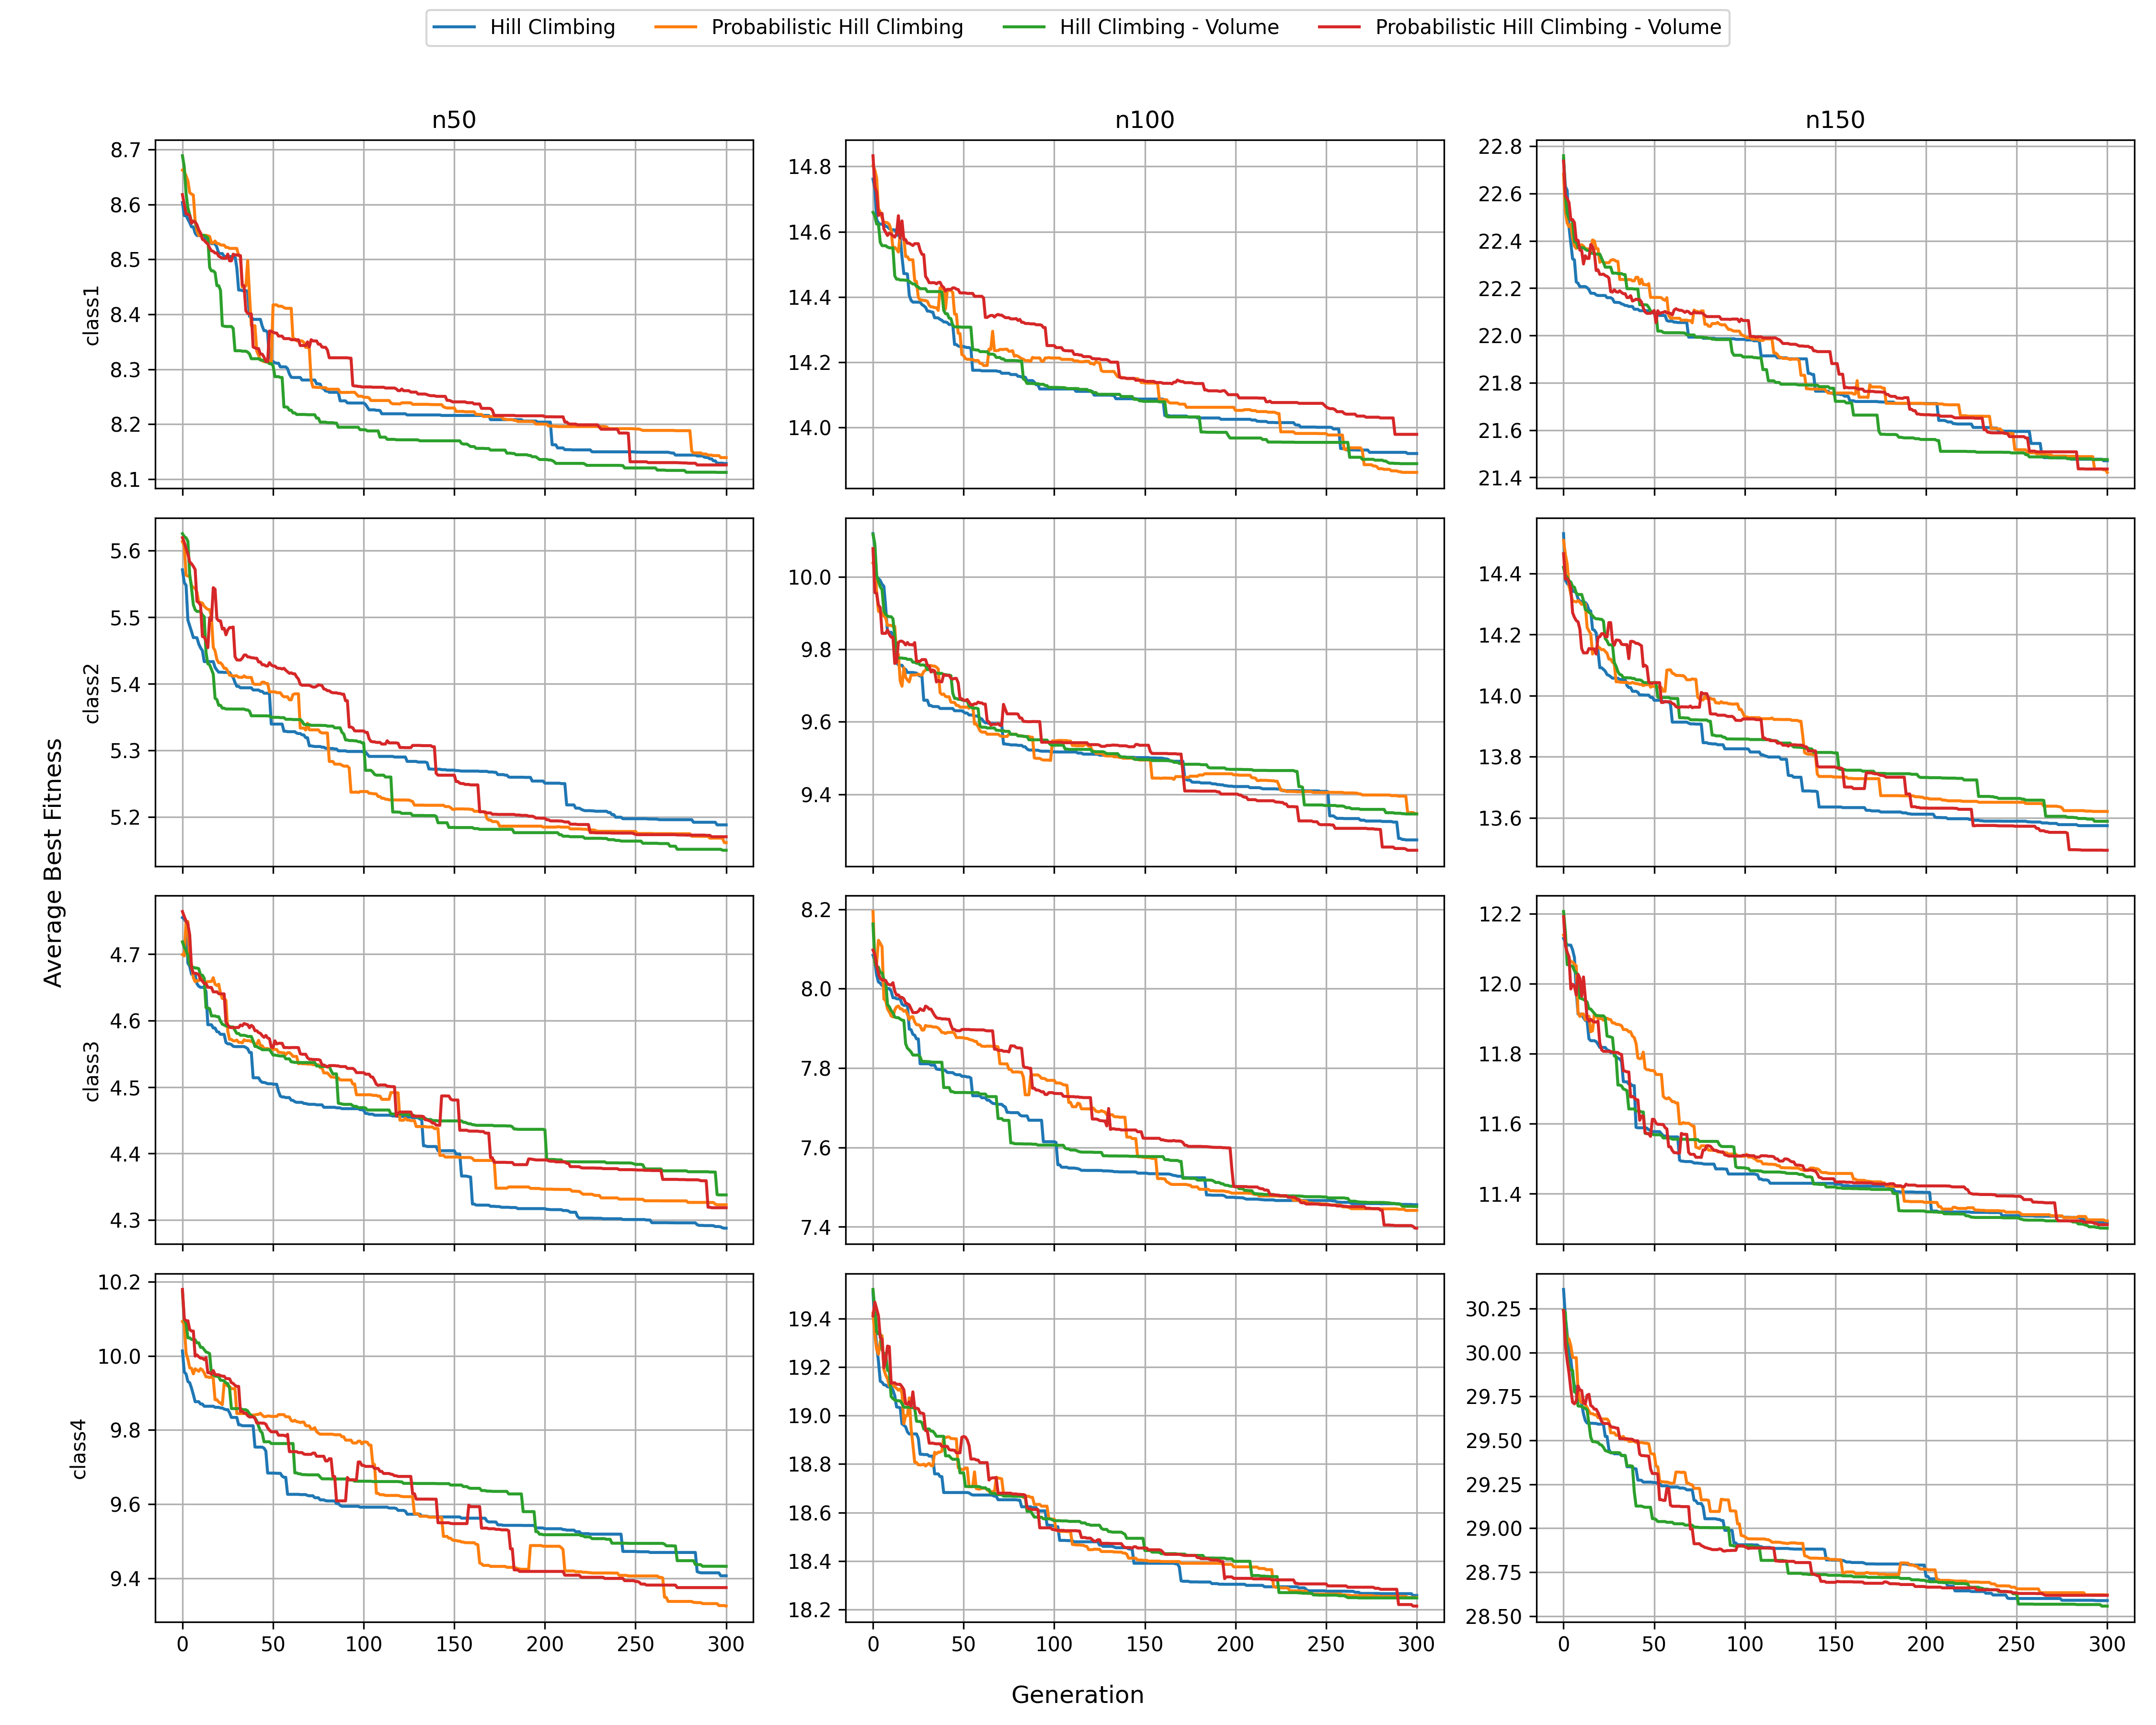
\includegraphics[width=1.2\textwidth]{img/hc-phc-volume.png}%
    }
    \caption{Comparison of probabilistic hill climbing and hill climbing with evolutionary and volume-based ordering.}
    \label{fig:hc-phc-volume}
\end{figure}


\subsection{Influence of Box Weights}

In this section, we examine how box weights affect the performance of the hill-climbing baseline. 
Unlike the elitist genetic algorithm, here we focus only on simple hill climbing with evolutionary ordering on the original, medium, and heavy datasets, since probabilistic hill climbing and volume-based ordering performed similarly or worse on the unweighted dataset. 
The comparison of the evolutionary progress across the three datasets is shown in Figure~\ref{fig:hc-weight-comparison}.
The comparison with the elitist algorithm and the lower bound is shown in Figures~\ref{fig:final-medium} and~\ref{fig:final-heavy}.

As expected, the elitist algorithm clearly outperforms hill climbing in most cases. 
The only notable exception is the heavy dataset, where the gap between hill climbing and the elitist algorithm is smaller in terms of final solution quality. 
However, this is mainly caused by the fact that the strong weight constraint significantly limits the space of feasible improvements, rather than by hill climbing achieving comparable search performance. 
Even in this case, the elitist algorithm converges substantially faster and reaches high-quality solutions earlier than hill climbing.

An interesting difference can be observed when comparing the original and medium datasets. 
For the elitist algorithm, these two datasets started from similar initial fitness values, but eventually converged to different final values because the weight constraint became more important during the search. 
For hill climbing, the situation is somewhat different: although the original and medium datasets also start from similar fitness values, they often end with similarly good solutions as well. 
This suggests that hill climbing does not explore the search space deeply enough for the weight constraint to become clearly dominant and to induce a noticeable change in the optimisation behaviour.

Overall, these results indicate that box weights have a stronger impact on the elitist genetic algorithm than on hill climbing, 
most likely because hill climbing is not sufficiently powerful to fully exploit the additional structure induced by the weights. 
At the same time, the heavy dataset imposes such a strong feasibility constraint that the gap between the hill-climbing baseline and the elitist method is the smallest in this case, although it remains substantial.

\begin{figure}[htbp]
    \centering
    \makebox[\textwidth][c]{%
    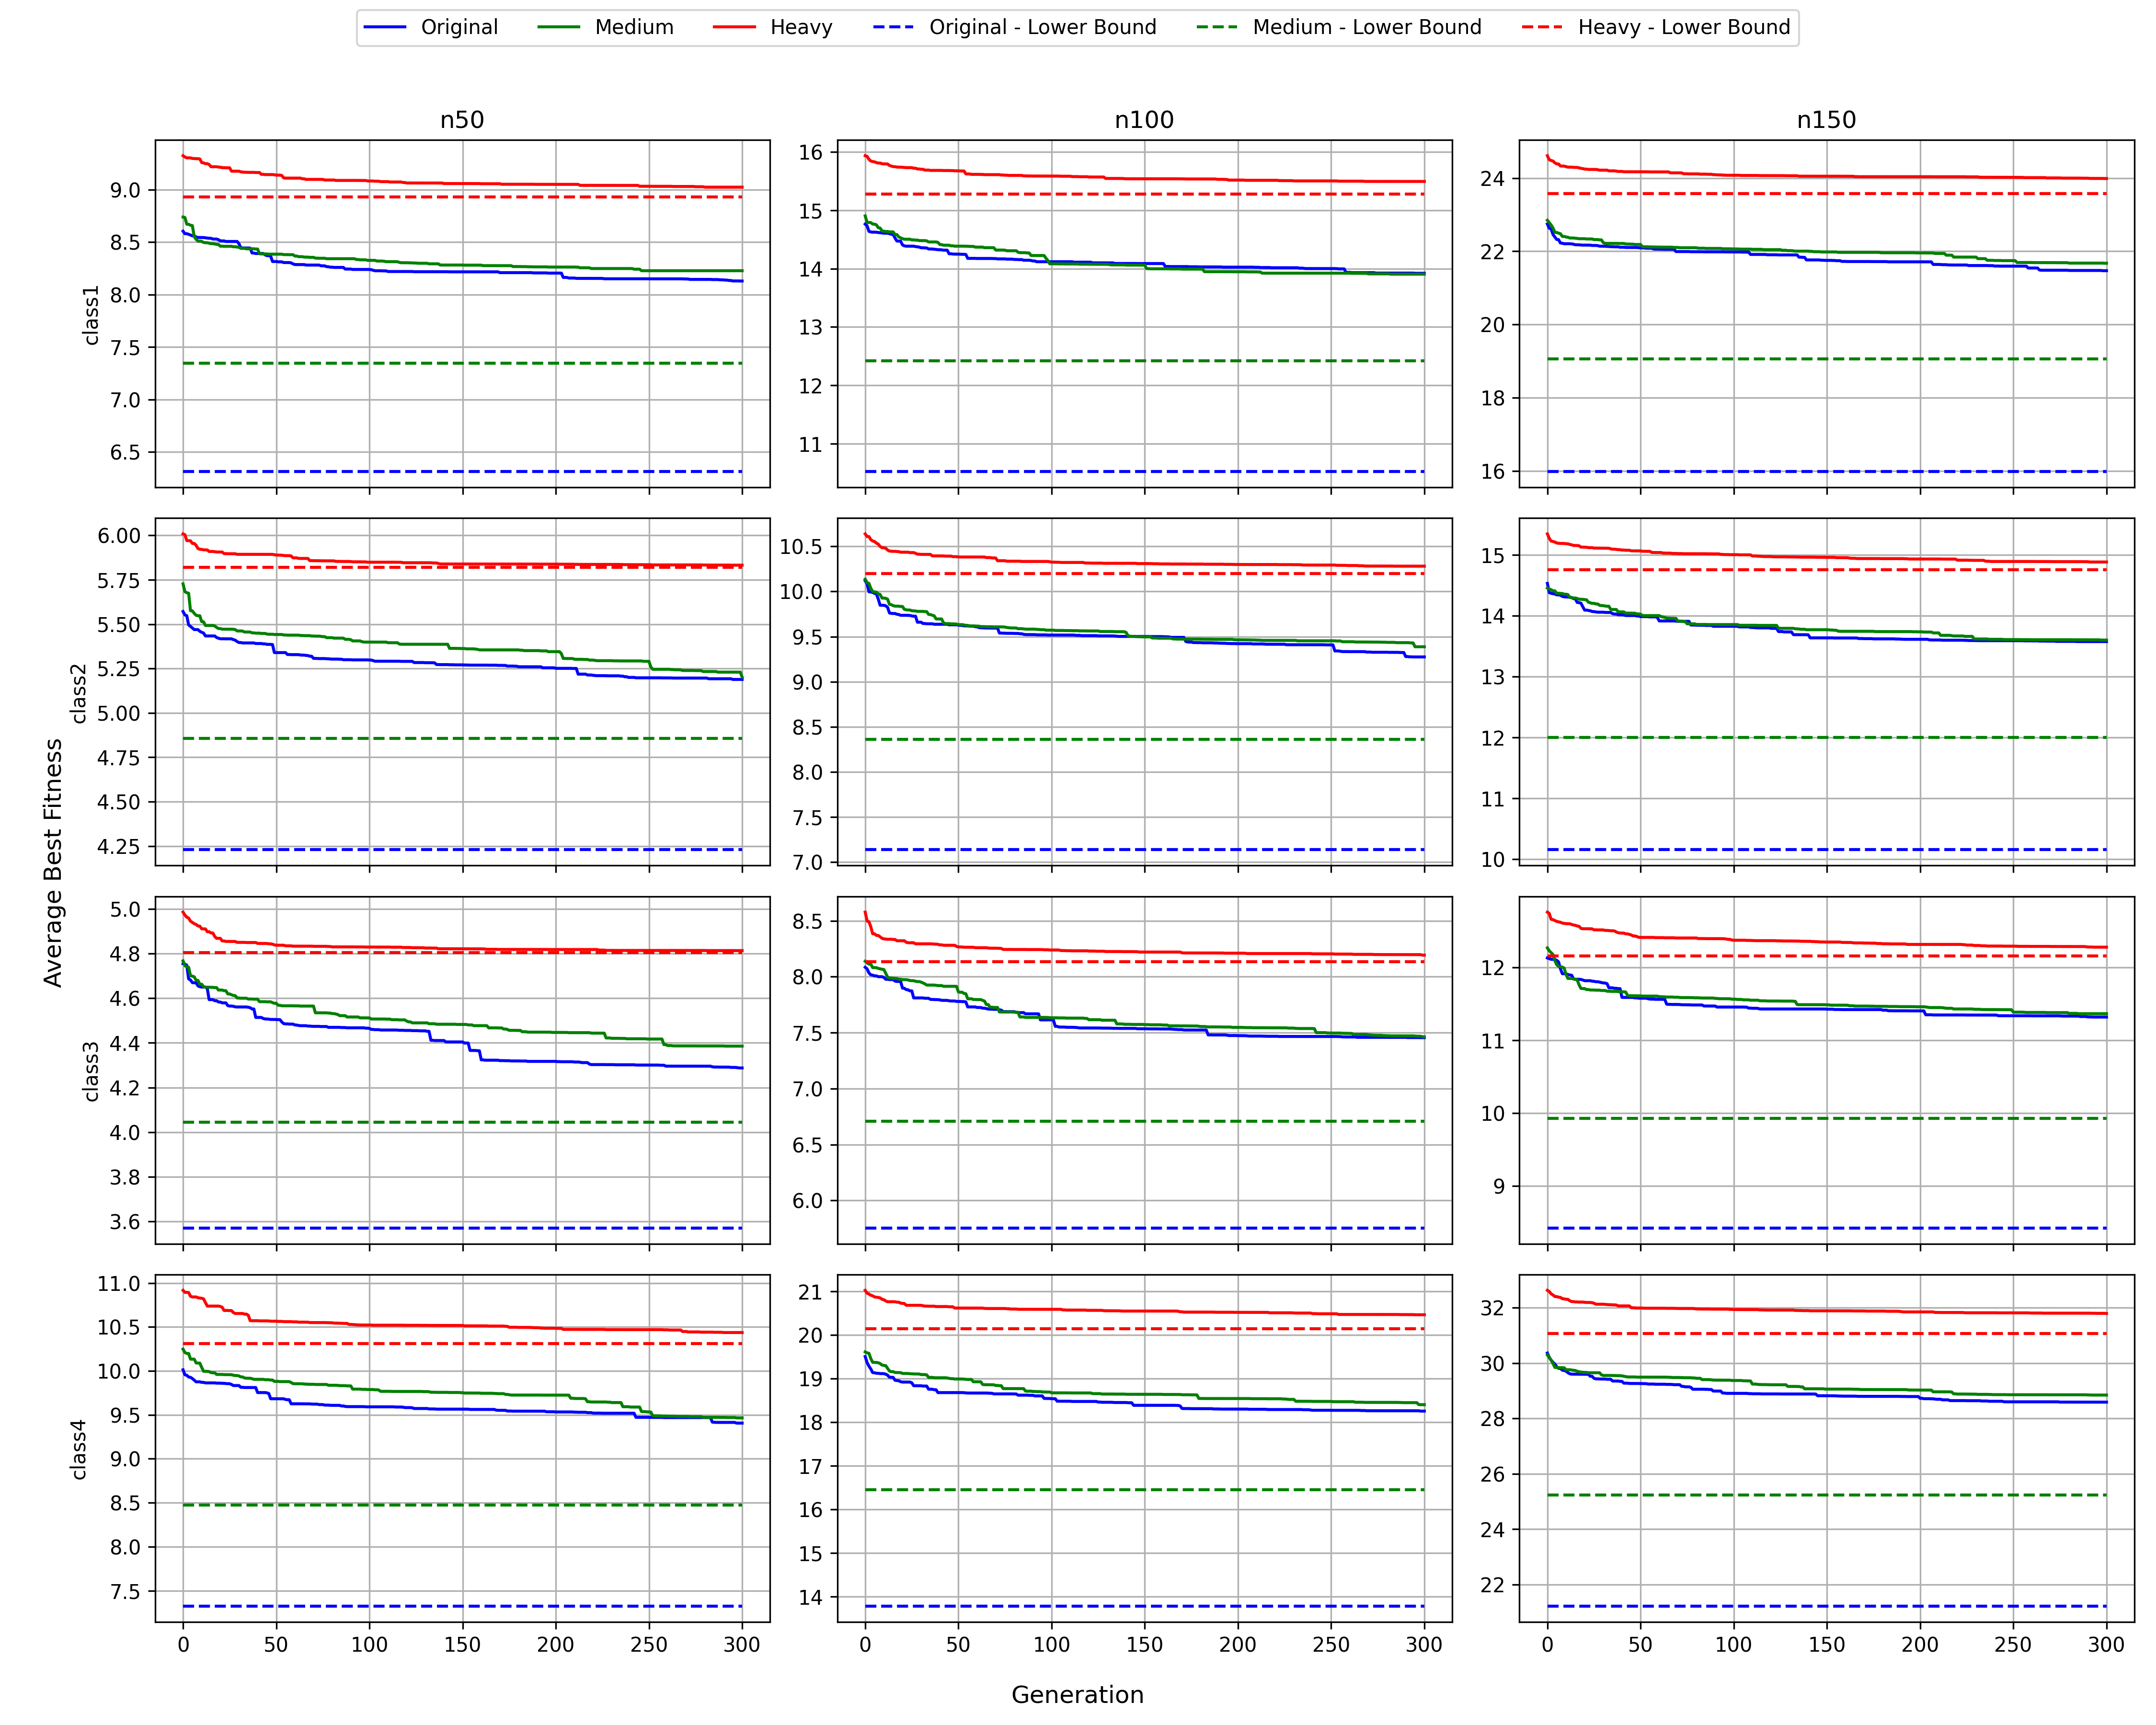
\includegraphics[width=1.2\textwidth]{img/hc-weights.png}%
    }
    \caption{Comparison of the evolutionary progress for hill climbing across the original, medium, and heavy datasets.}
    \label{fig:hc-weight-comparison}
\end{figure}

\begin{figure}[htbp]
    \centering
    \makebox[\textwidth][c]{%
        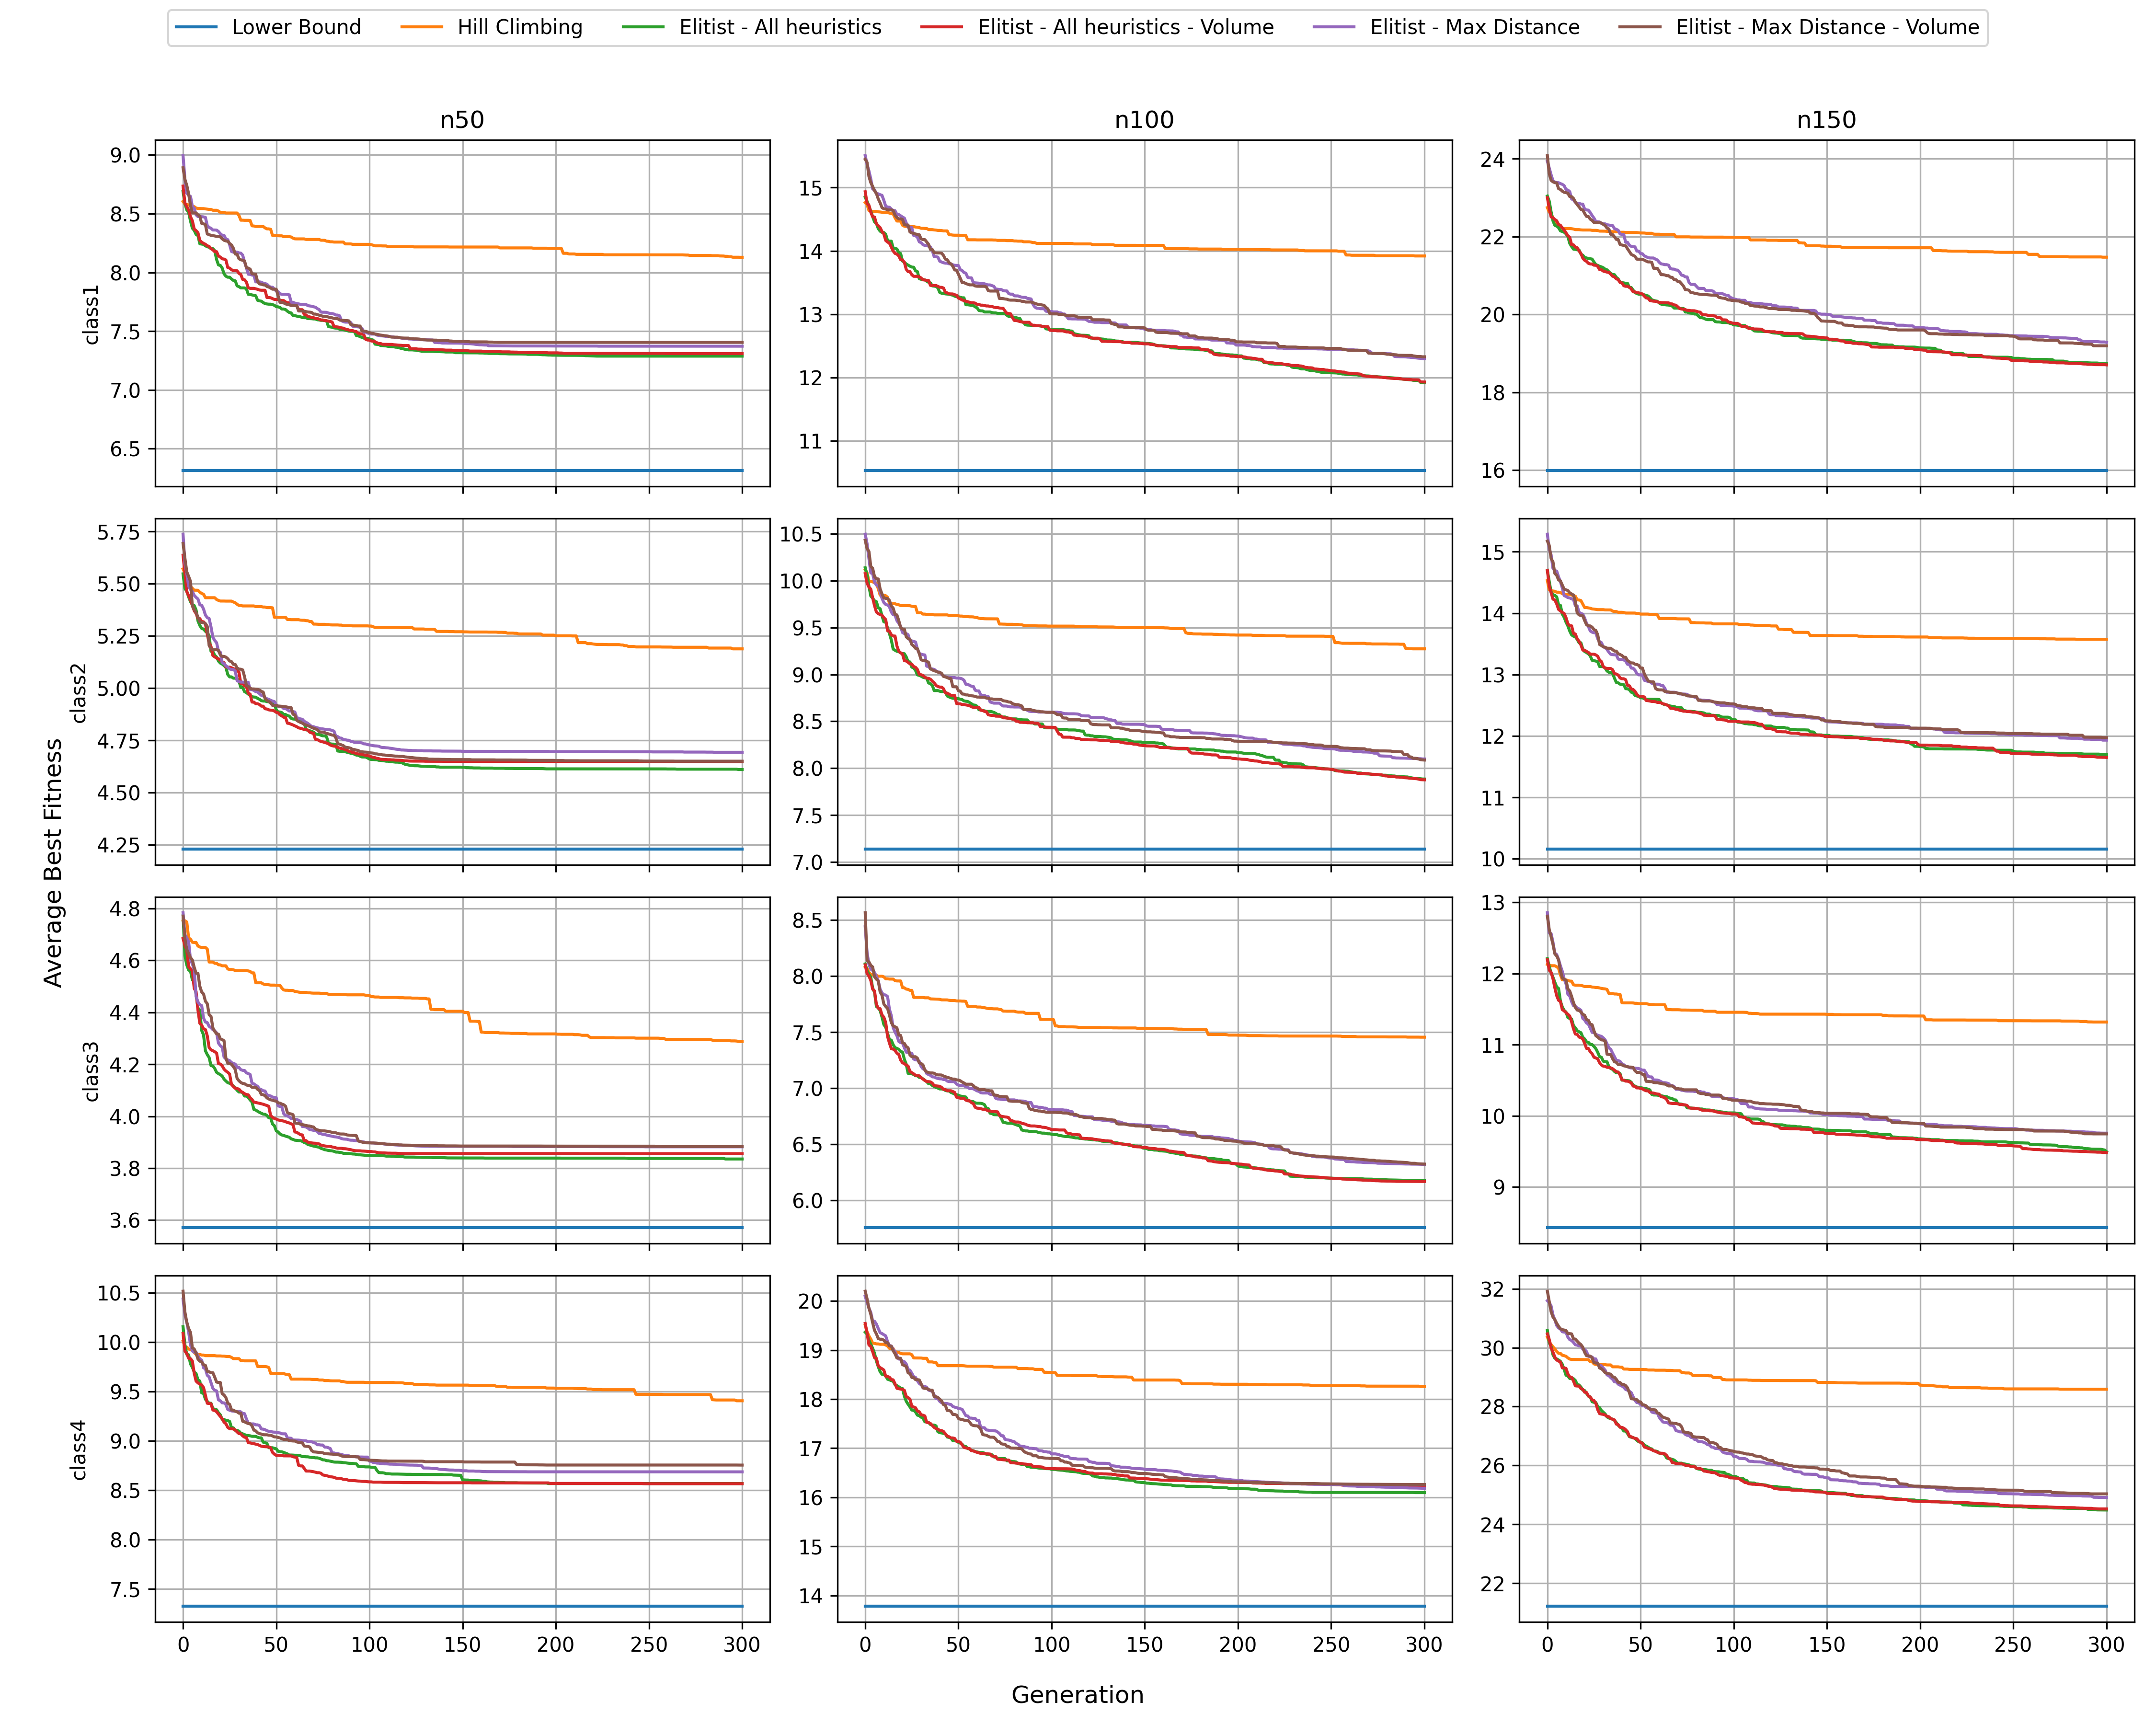
\includegraphics[width=1.2\textwidth]{img/comparison-original.png}%
    }
    \caption{Evolutionary progress for all four settings on the unweighted dataset 
    using the elitist algorithm, including the lower bound and the hill-climbing baseline.}
    \label{fig:final-original}
\end{figure}

\begin{figure}[htbp]
    \centering
        \makebox[\textwidth][c]{%
        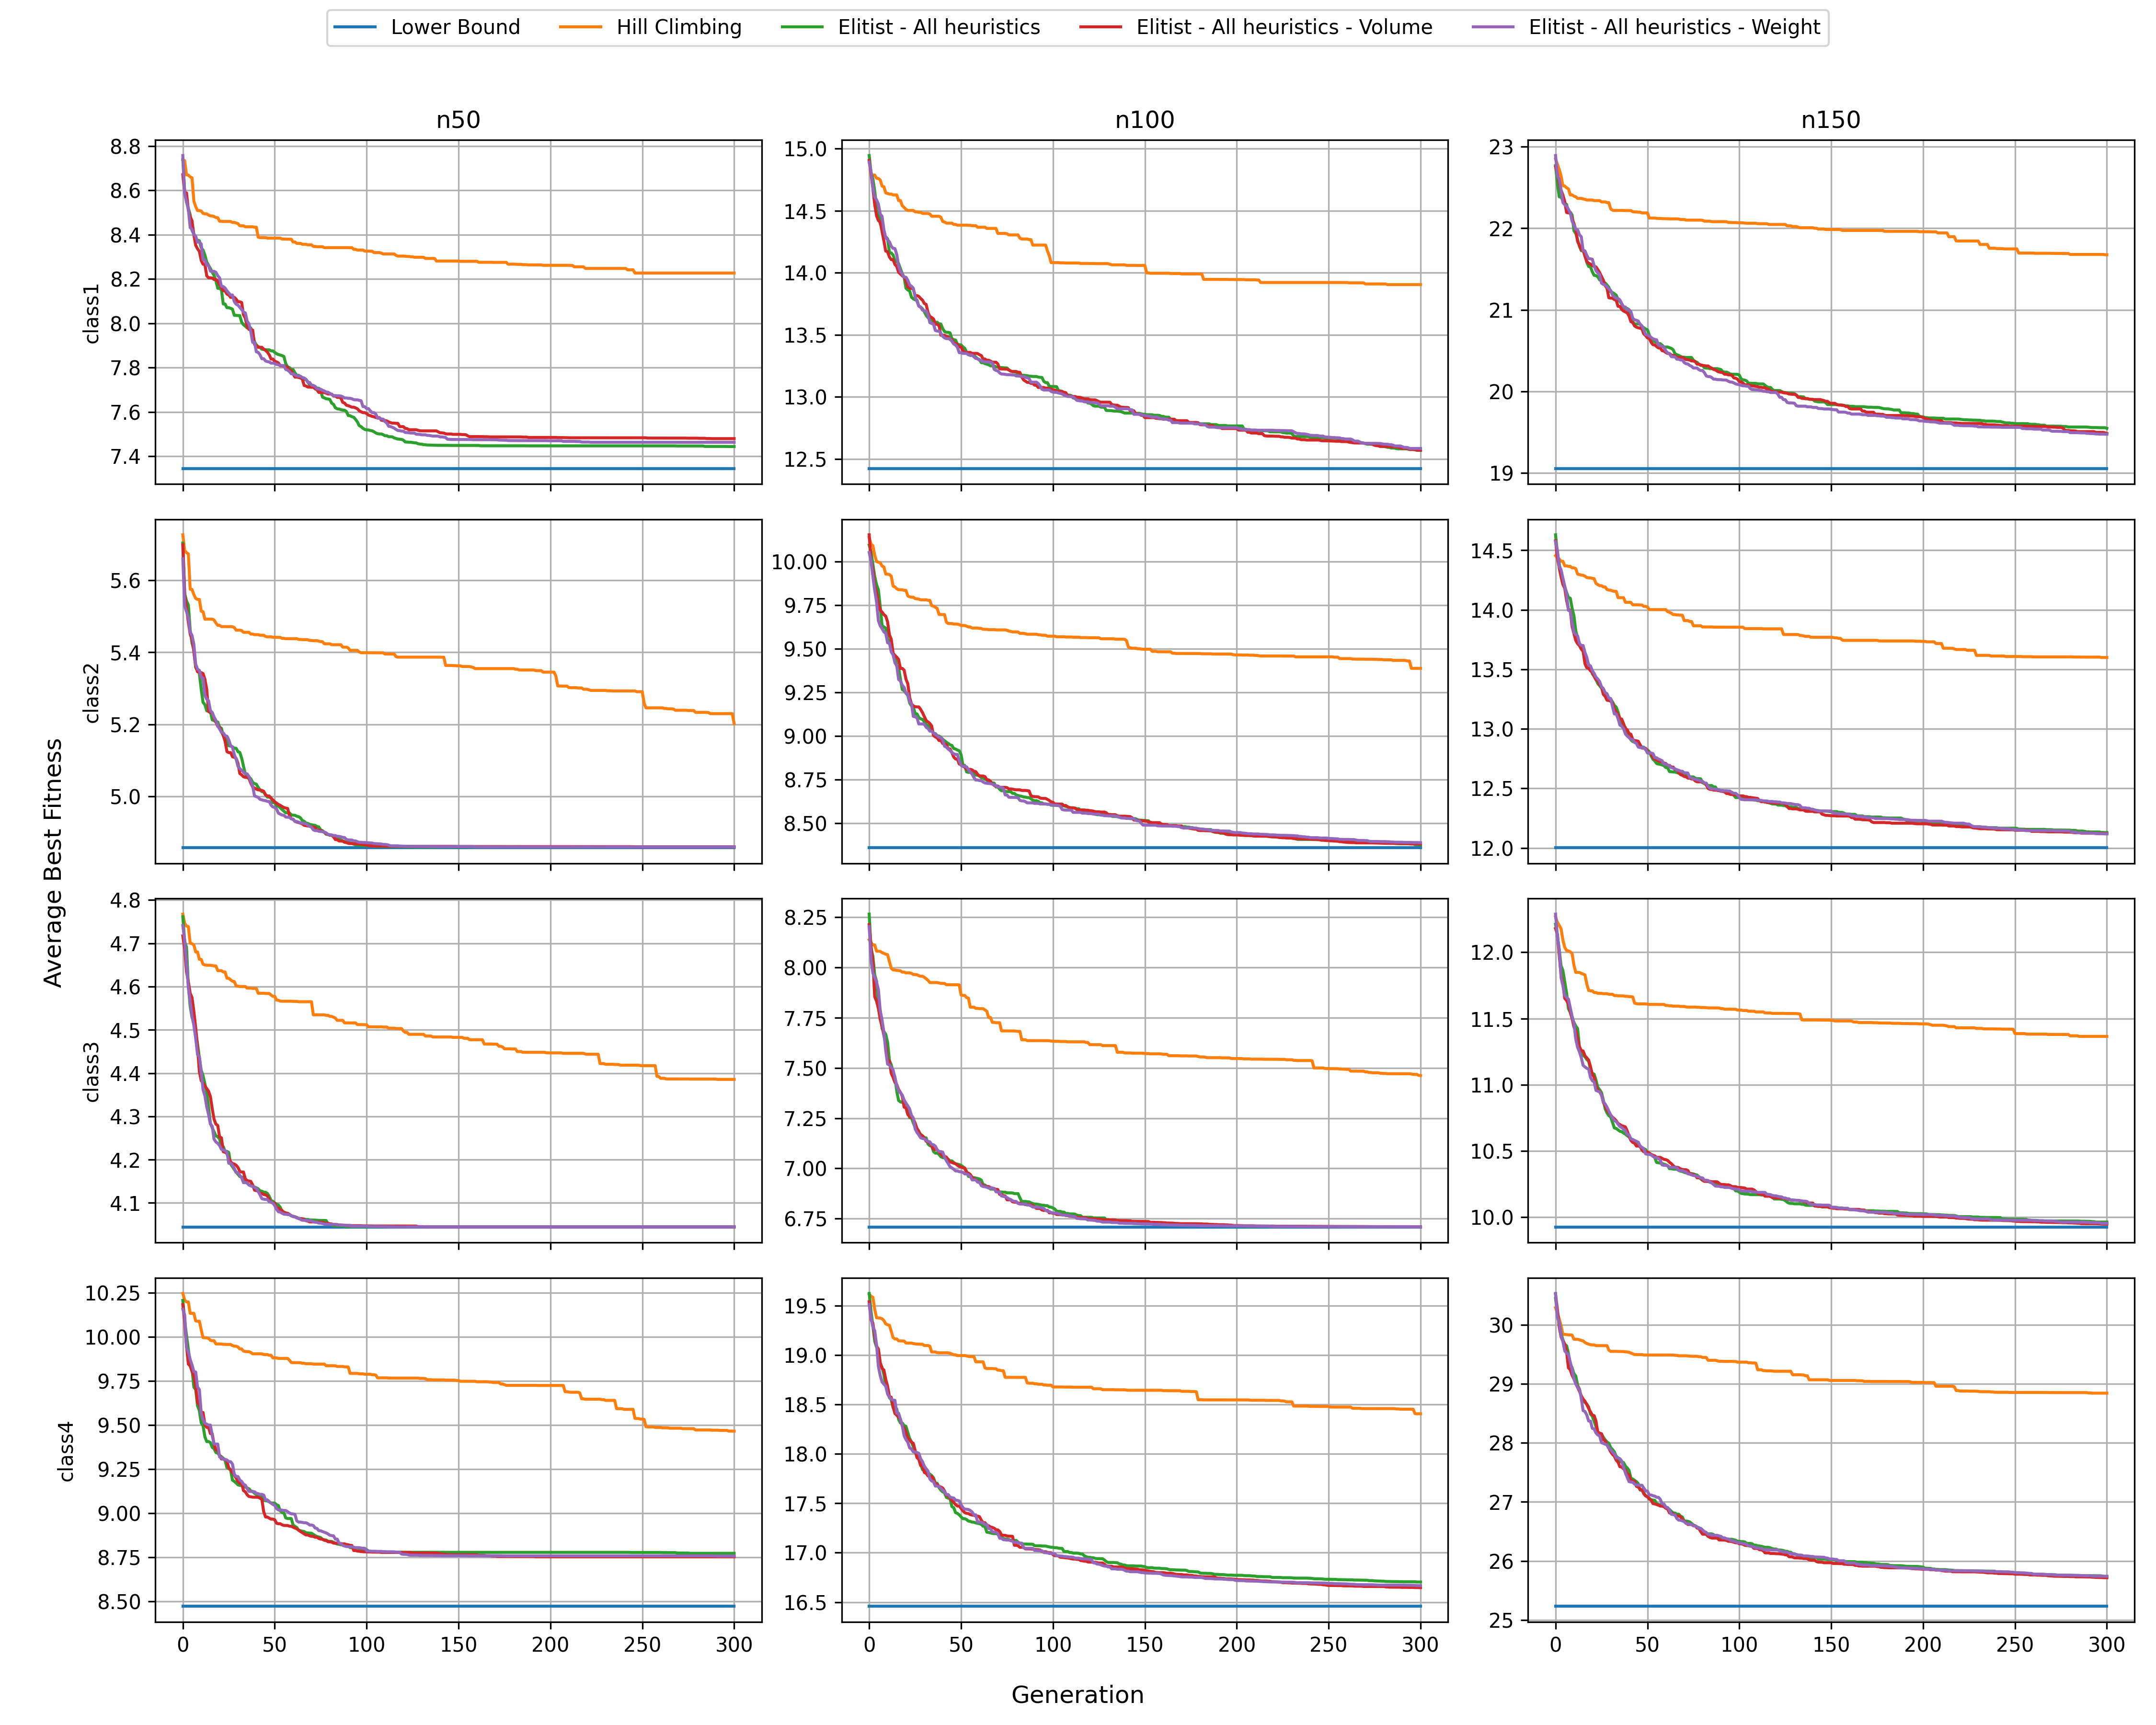
\includegraphics[width=1.2\textwidth]{img/comparison-medium.png}%
    }
    \caption{Evolutionary progress for different ordering strategies on the medium dataset 
    using the elitist algorithm, including the lower bound and the hill-climbing baseline.}
    \label{fig:final-medium}
\end{figure}

\begin{figure}[htbp]
    \centering
    \makebox[\textwidth][c]{%
        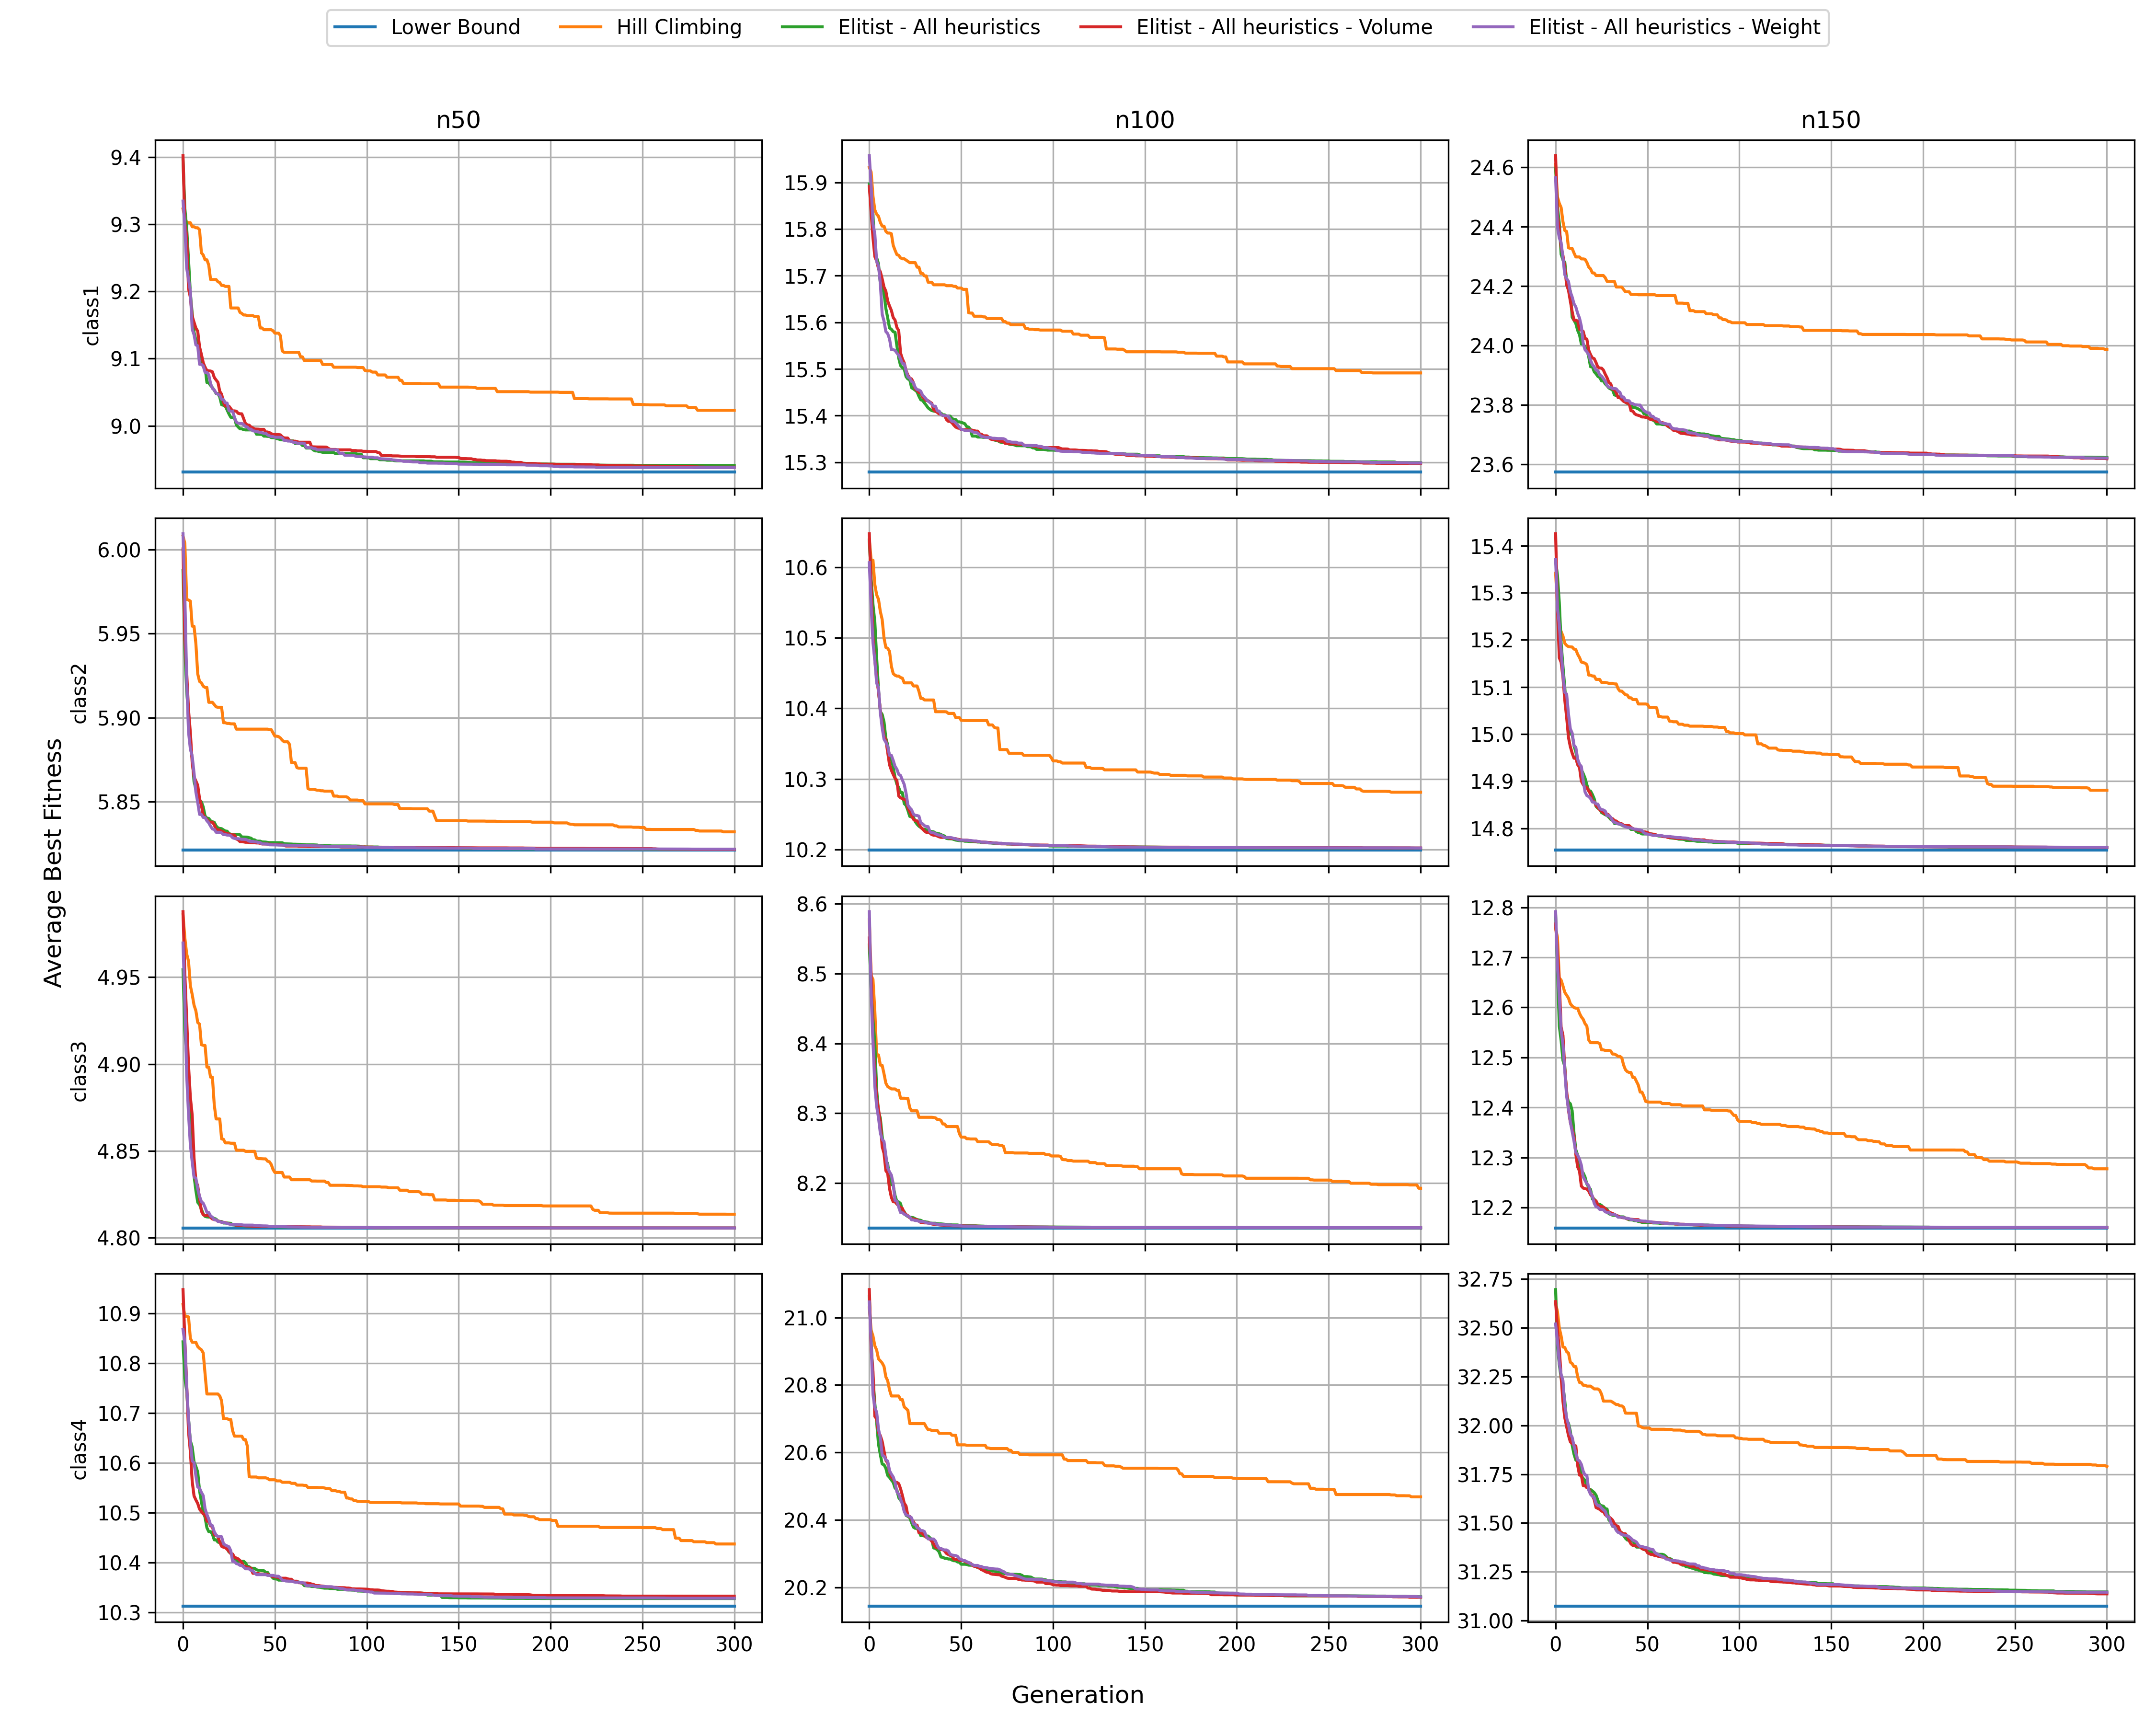
\includegraphics[width=1.2\textwidth]{img/comparison-heavy.png}%
    }
    \caption{Evolutionary progress for different ordering strategies on the heavy dataset 
    using the elitist algorithm, including the lower bound and the hill-climbing baseline.}
    \label{fig:final-heavy}
\end{figure}

